%************************************************
\chapter{Significance Weighted Principal Component Analysis}\label{ch:swpca}
%************************************************
Multicentre studies with structural \ac{MRI} and functional \ac{MRI} (f\ac{MRI}) are increasingly common, allowing for recruitment of larger populations in shorter periods of time. However, the use of images acquired at different sites still poses a major challenge. In addition to logistical difficulties, such as regulatory approvals and data protection, a number of technical and methodological issues can potentially affect the resulting maps, introducing undesired intensity and geometric variance. This issue has been addressed in other neurological conditions, such as \ac{AD} \cite{Jovicich2006,Stonnington2008}, where group differences are well known, and demonstrating that the impact of a correction for site on the resulting neurobiological differences is relatively small. However, these effects have a stronger impact in psychiatric conditions where the atypical radiological signs on \ac{MRI} are often subtle and require large samples of patients to observe on-average differences relative to control samples. Recent meta-analyses point to differences being inconsistently reported in schizophrenia \cite{friedman2006report,Turner2013}, psychosis \cite{Clementz2015,Wang2015}, and \ac{ASD} (using the multi-centre ABIDE database) \cite{haar2014anatomical}

These inconsistencies can arise from a variety of variance sources, ranging from the multi-level (phenotypic, neurobiological, and etiological) heterogeneities of the conditions to technical issues that include differences in scanner make, model, manufacturer, static field strength, field inhomogeneities, slew rates and image reconstruction \cite{VanHorn2009}, as well as acquisition problems such as within-acquisition participant head motion. Field inhomogeneities are a source of misinterpretation of the data even when the same \ac{MRI} system manufacturer and model are used \cite{VanHorn2009}. Furthermore, results in \cite{Pearlson2009} demonstrate that a single scanner can change with time, which makes some widely used strategies, for example collecting controls first and patients later, a flawed approach. Recent neuroimaging research on \ac{ASD} \cite{haar2014anatomical} has shown that, while analyses performed on a particular database (acquired on a single platform) could yield coherent regions, the atypical structures are often inconsistent across the wider literature using different databases. Therefore, new methodologies focused on reducing multi-site variance may be potentially helpful in increasing the power to identify the characteristic neurobiological signature of autism, should there be one. 

A number of approaches have been proposed to reduce between-site variance. Geometric distortions caused by magnetic fields inhomogeneities have been widely studied \cite{Jovicich2006,Stonnington2008}. Furthermore, there exist a number of diffeomorphic registration algorithms, such as DARTEL \cite{Ashburner2007} or ANTS \cite{Avants2010}, intended to reduce inter-subject—and by extension, inter-site—variations. In the case of intensity variance, the issue has already been addressed in the \ac{MRC-AIMS} database by leveraging sMRI sequences that yield quantitative estimates of relaxation times \cite{deoni2008standardized} which have been demonstrated to reduce single-site effects compared to weighted sequences. However, images acquired using this technique still yield between-site differences \cite{Suckling2014}.

To address the problem of intensity variance and improve the homogeneity of the images across different sites, we have proposed a new post-acquisition methodology that enhances derived maps (e.g. grey or white matter volumes) by means of ameliorating site effects \cite{Martinez-Murcia2016a}. This method, called \acf{SWPCA}, can be applied as part of pre-processing before computing whole-brain or regional statistical analysis. The algorithm proceeds by performing a \ac{PCA} over the whole database of images and later computing the statistical significance of each component in relation to a categorical variable, in this case the acquisition site. This information is used to reconstruct the datasets using a weighted strategy that effectively reduces intensity inhomogeneities due to site effects.

\section{\acf{SWPCA}}
The \acf{SWPCA} is an algorithm to reduce undesired intensity variance introduced by multi-site image acquisition. \ac{SWPCA} takes any dataset of pre-processed images and decomposes them into their variance components to then provide a corrected dataset where the undesired variance has been reduced. To do so, \ac{PCA} is applied to each modality in turn to obtain the component scores and component loadings. Since \ac{PCA} is a data-driven approach, it was only used to decompose the source images, and after this procedure, a one-way \ac{ANOVA} estimates the relation between each variance component and a given categorical variable, in our case, the acquisition site. The between-site variability in the variance component is then identified by its corresponding \textit{p}-value. Finally, these \textit{p}-values are transformed into a weighting matrix  $\boldsymbol\Lambda$ that weights the influence of each variance component in a final \ac{PCA} reconstruction of the corrected maps. The procedure is summarized in Figure~\ref{fig:swpcaschema}. There is also a python class for performing \ac{SWPCA} at \url{https://github.com/SiPBA/swpca}. 

\begin{figure}
\centering
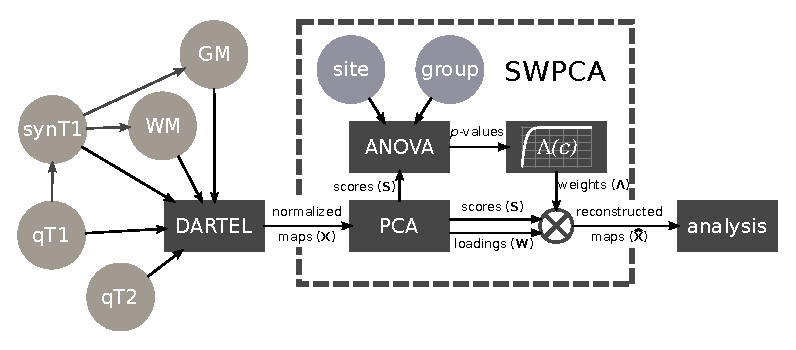
\includegraphics[width=\linewidth]{Graphics/ch7/FIGURE01}
\caption[Summary of the \acs{SWPCA} algorithm, along with its context in the pipeline used in this article.]{Summary of the \ac{SWPCA} algorithm, along with its context in the pipeline used in this article. Circles represent the input data, both images (green shading) and class (group and acquisition site, purple shading). Rectangles represent the different procedures applied, comprising the DARTEL normalization and registration, the different steps contained in \ac{SWPCA}, \ac{ANOVA} and obtaining the weighting function $\Lambda(c)$- and the subsequent analysis.}
\label{fig:swpcaschema}
\end{figure}


\subsection{\acf{PCA}}\label{sec:pca}
The first step in the \ac{SWPCA} algorithm is to perform a \ac{PCA} decomposition
of the dataset into a set of orthogonal components that model the
variance present in the images. 

\ac{PCA} is a statistical procedure that uses an orthogonal transformation to convert a set of observations $\mathbf{X}$ of possibly correlated variables, where $\mathbf{X}$ is a $N\times K$ matrix, with $N$ participants (in this case, with one image per participant) and $K$ the number of voxels, into a set of $K$ linearly uncorrelated variables called Principal Components (PC, also known as component loadings or the mixing matrix)  $\mathbf{W}$ of size $K\times K$ whose linear combination using a vector of component scores  $\mathbf{s}_{N}$ can perfectly recompose each image. 

Intuitively, \ac{PCA} defines a new space where the first spatial direction is defined so that it explains the maximum variance in the data. The subsequent directions will try to explain the remaining variance in decreasing order. The set of these component scores  $\mathbf{S}$ (size $N \times K$) is estimated as:

\begin{equation}\label{eq:pcabasic}
	\mathbf{S}=\mathbf{X}\mathbf{W}^T
\end{equation}
where the columns of $\mathbf{W}$ contain the eigenvalues of $\mathbf{X}^T\mathbf{X}$, the empirical covariance matrix of $\mathbf{X}$. 

This transformation computes a sequence of PCs, maximally explaining the variability of the data while maintaining orthogonality between components. This is done, ideally, by obtaining the \ac{EVD} of the empirical covariance matrix of the data. The mixing matrix $\mathbf{W}$ is then defined as the set of eigenvectors obtained after applying the \ac{EVD} to the covariance matrix of the data $\mathbf{X}^T\mathbf{X}$ (assuming that the column mean was substracted from the data) so that: 
\begin{equation}\label{eq:covariance}
\mathbf{X}^T\mathbf{X} = \mathbf{W}\boldsymbol\Lambda\mathbf{W}^T
\end{equation}
where $\boldsymbol\Lambda$ is a diagonal matrix whose diagonal elements contain the eigenvalues of each principal component, and the mixing matrix $\mathbf{W}$ contains the eigenvectors. 

The most popular approach to obtaining the decomposition takes advantage of some analogies between the \ac{SVD} of $\mathbf{X}$ and the \ac{EVD} of $\mathbf{X}^T\mathbf{X}$. Since the \ac{EVD} is often more computationally expensive, the \ac{SVD} approach is often used. \ac{SVD} performs the decomposition:
\begin{equation}
\mathbf{X} = \mathbf{U} \boldsymbol{\Sigma} \mathbf{V}^* 
\end{equation}
where  $U$ is an $N\times N$ orthogonal matrix,  $\boldsymbol\Sigma$ is a $N\times K$ diagonal matrix with non-negative real numbers on the diagonal, and the $K\times K$ unitary matrix  $\mathbf{V}^*$ denotes the conjugate transpose of the $K\times K$ unitary matrix $\mathbf{V}$.
Using that decomposition, the covariance matrix 
\begin{equation}
\mathbf{X}^T\mathbf{X} = \mathbf{V}\boldsymbol\Sigma\mathbf{U}^T\mathbf{U}\boldsymbol\Sigma\mathbf{V}^T = \mathbf{V}\boldsymbol\Sigma^2\mathbf{V}^T
\end{equation}
which, comparing with Equation \ref{eq:covariance}, shows that we can obtain the mixing matrix as $\mathbf{W} = \mathbf{V}$, the eigenvalues $\boldsymbol\Lambda = \boldsymbol\Sigma^2$, and the transformed samples of Eq.~\ref{eq:pcabasic} can be rewritten as $\mathbf{S} = \mathbf{X}\mathbf{W} = \mathbf{U}\boldsymbol{\Sigma}$. 

We obtained both the component scores and estimates of the `eigenbrains' $\mathbf{W}$. In \ac{PCA}, the maximum variability in the data (information) is contained within the first components, and the remaining can be considered noise. Therefore, for this chapter, the truncated form of \ac{SVD} was used such that only the first $C$ components were considered, where most of the variability of the data was concentrated:

\begin{equation}
	\mathbf{S}_C = \mathbf{U}_C \boldsymbol{\Sigma}_C = \mathbf{X}\mathbf{W}_C
\end{equation}

where  $\mathbf{S}_C$ is the set of component scores using the first $C$ components (size $N\times C$). To achieve reasonable performance with minimal information loss, it was assumed that the number of components was the same as the number of images, $C=N$. Thus, a partial reconstruction of the original signal could be undertaken:

\begin{equation}\label{eq:swpcareconst}
	\hat{\mathbf{X}}=\mathbf{S}_C \mathbf{A}_C
\end{equation}

where  $\mathbf{A}_C$ is the pseudoinverse of the truncated matrix of component loadings  $\mathbf{W}_C$, and  $\hat{\mathbf{X}}$ is the reconstructed set of images.


\subsection{One-Way \acf{ANOVA}}
The estimated PCs effectively model the variability of the image dataset. The next step was to assess each PC as a source of inter-site variance with one-way \acf{ANOVA}. \ac{ANOVA} estimates the $F$-statistic, defined as the ratio between the estimated variance within groups and the variance between groups:
\begin{equation}
F=\frac{M{S}_{\mathit{within}}}{M{S}_{\mathit{between}}}=\frac{S{S}_{\mathit{within}}/(G-1)}{S{S}_{\mathit{between}}/(K-G)}=\frac{\sum
	_{i}{{n}_{i}{\left({\bar{{Y}}}_{i}-\bar{{Y}}\right)}^{2}/{\left(G-1\right)}}}{\sum
	_{\mathit{ij}}{{\left({Y}_{\mathit{ij}}-\bar{{{Y}_{i}}}\right)}^{2}/{\left(K-G\right)}}}
\end{equation}

Where  $M{S}_{\mathit{within}}$ \ and  $M{S}_{\mathit{between}}$ are the mean squares within- and between-groups respectively, $G$ is the number of separate groups (in our case, two),  $\bar{Y}$ is the sample mean of a certain feature (in our case, the sample mean of all $K$ values of a given component score),  ${\bar{Y}}_{i}$ is the sample mean of the features belonging to group $i=1\dots G$, ${Y}_{\mathit{ij}}$ is the $j_{th}$ observation of a feature belonging to group \textit{i} and  ${n}_{i}$ is the number of participants in the  $i_{th}$ group. The $F$-distribution allows an easy computation of $p$-values, given the number of groups and degrees of freedom. The $F$-statistic and $p$-values were computed independently for each component score and acquisition site, and then used in the \ac{SWPCA} algorithm.

\subsection{Weighting Function}
To obtain a set of corrected maps, a new signal matrix of all maps of the same modality,  $\widehat{\mathbf{X}}$, was estimated with the influence of the PCs with variance related to acquisition site, assessed via the $p$-values, reduced. To do so, equation~\ref{eq:swpcareconst} was modified to include a square matrix $\boldsymbol\Lambda$ (dimension $C\times C$) whose diagonal contains a weight ${\lambda }_{c}$ for each component that depends on its $p$-value; that is,

\begin{equation}
	\widehat{\mathbf{X}} = \mathbf{S}\boldsymbol{\Lambda}\mathbf{A}
\end{equation}

The computation of each ${\lambda }_{c}$, for each component, was performed using the Laplace distribution, modified so that the weights were on the interval [0, 1]:
\begin{equation}
	\lambda_{c}(p_c, p_{th}) = 1-e^{\frac{-p_c}{p_{th}}} \quad \forall p_c \in \left[0,1\right]
\end{equation}

where  ${p}_{c}$ is the statistical significance of the $c_{th}$ component with respect to the acquisition site and ${p}_{th}$ is the statistical threshold for significance; that is,  ${p}_{th}$=0.05. A plot of the univariate weighting function $\lambda_c(p_c,p_{th})$ can be found in Figure~\ref{fig:swpcasweigthing}. This weighting ensured that most of the components of variance that are not related to the acquisition site are kept unchanged, while at the same time it strongly reduces the influence of components with $p$-values less than the threshold. 

\begin{figure}
	\centering
	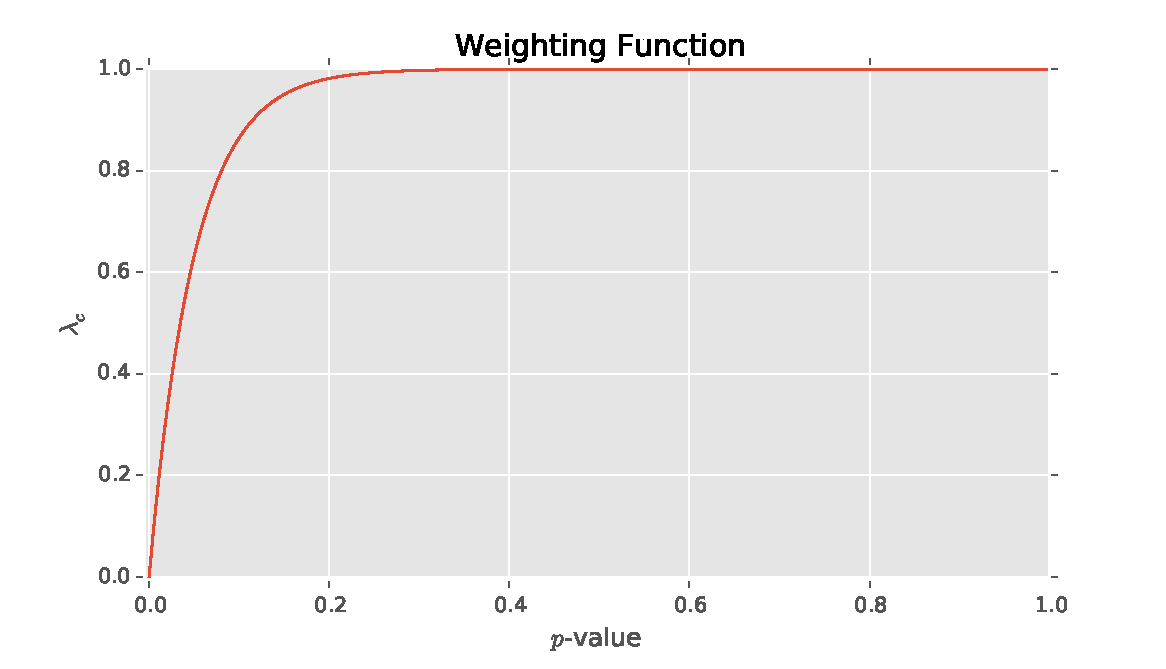
\includegraphics[width=0.6\linewidth]{Graphics/ch7/weighting2}
	\caption[Weighting function $\Lambda_c(p_c,p_{th})$ used in \acs{SWPCA}.]{Weighting function $\Lambda_c(p_c,p_{th})$ used in \ac{SWPCA}.}
	\label{fig:swpcasweigthing}
\end{figure}

This procedure is illustrated in Figure~\ref{fig:swpcaboxplot}, where a boxplot of the distribution of the first four principal component scores is shown. Since we have assumed that substantial differences imply a bigger influence of the acquisition site on the portion of variance modelled by that component, the resulting weight is reduced, and the contribution of that component to the reconstructed signal will be smaller. After computing all weights, most of the sources that are related to the acquisition site (for example, the second and third components with respectively $\lambda_2=0$ and $\lambda_3=6.14E-6$) have been parsed out while keeping all other sources of variance.

\begin{figure}
	\centering
	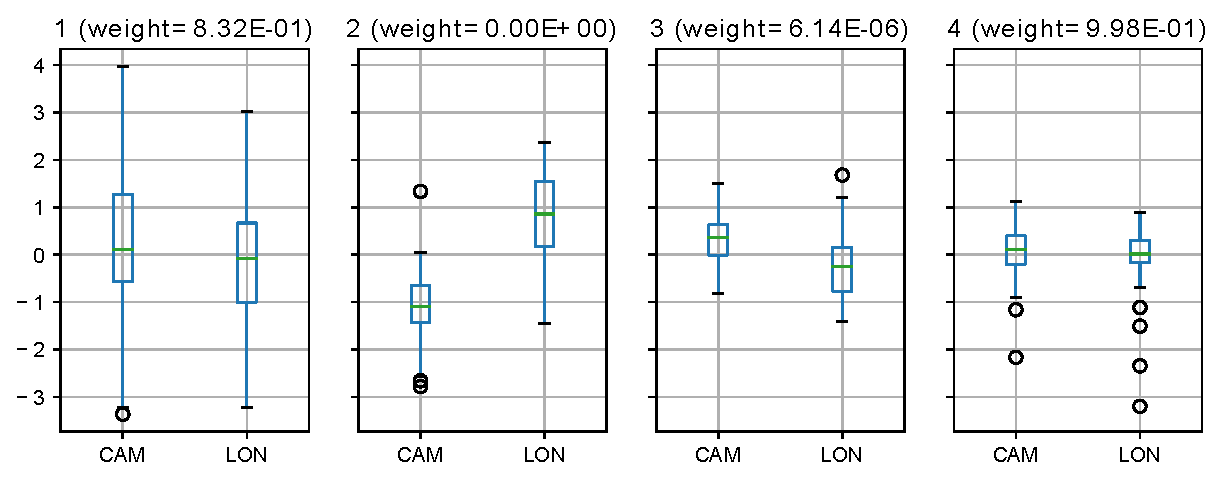
\includegraphics[width=\linewidth]{Graphics/ch7/FIGURE02}
	\caption[Box-plot of the distribution of the component scores at each site of the \aimsmri{} dataset (see Sections~\ref{sec:swpcaAIMSresults} and \ref{sec:aims-mri}) in the four first components.]{Box-plot of the distribution of the component scores at each site of the \aimsmri{} dataset (see Sections~\ref{sec:swpcaAIMSresults} and \ref{sec:aims-mri}) in the four first components. We assume that bigger differences between distributions imply a bigger influence of the acquisition site on the portion of variance modelled by that component and therefore, to parse out those differences, the resulting weight will be smaller.}
	\label{fig:swpcaboxplot}
\end{figure}

\origsection{Evaluation of \acs{SWPCA}}\label{sec:swpcaEval}
To validate the effects of the \ac{SWPCA} algorithm on the inter-site variance, three experiments were undertaken to assess the reduction of the undesired site variance in the original datasets, and its impact on the between-group signal. Two kind of analysis have been performed: a characterization of voxel-wise differences, and a classification analysis. 

Voxel-wise differences between groups were characterized using \ac{VBM} \cite{Ashburner2000}, comprising preprocessing (registration, smoothing) and mass-univariate $t$-test on the smoothed maps from each modality. \ac{SWPCA} is included (when needed) in this pipeline as a plug in, after the smoothing and before the hypothesis testing. Permutation testing assessed the significance of the relationship between the tested and target variables. A max-type procedure was used to obtain family-wise, whole-brain corrected \textit{p}{}-values \cite{Freedman1983}. Additionally, a \acf{CBM}, based on Source Based Morphometry (SBM) \cite{Xu2009} was used. This procedure provided Z-maps for visual inspection comparable to those obtained in \ac{VBM}, by selecting component loadings $\mathbf{W}$, scaling them to unit standard deviation and weighting their contribution to the final map with their statistical significance, computed using the same permutation inference as in \ac{VBM}. 

A classification analysis was undertaken using a common classification pipeline \cite{Khedher2015} consisting of preprocessing, feature extraction via \ac{PCA} and \ac{SVC} classification. \ac{SWPCA} is used as a plug-in here as well, after the preprocessing and before the feature extraction step. The classification was validated using stratified 10-fold cross-va\-li\-da\-tion \cite{Kohavi1995}. 

For each modality independently, the following experiments were performed: 
\begin{itemize}
	\item \textbf{Experiment 1}: To demonstrate the ability of the \ac{SWPCA} algorithm	to reduce undesired effects due to acquisition site, the \ac{PCA} + \ac{SVC} pipeline was applied to the datasets labelled by acquisition site. Classification accuracy was compared to datasets with and without \ac{SWPCA}. \ac{VBM} was then applied to identify the spatial location of the between-site differences. This was undertaken on the whole database (\all{}), and subgroups containing only \ac{ASD} or \ac{ASD} participants. 
	
	\item \textbf{Experiment 2}: The discrimination ability of each modality, acquired at different sites was assessed by classification performance of individuals from London (\lon{}) and Cambridge (\cam{}) was separately assessed, using group (\ac{ASD} and \ac{CTL}) as the labels. 
	
	\item \textbf{Experiment 3:} To assess the impact of \ac{SWPCA} on the datasets when characterizing the differences between \ac{ASD} and \ac{CTL} groups, the classification pipeline comprising \ac{PCA} + \ac{SVC}, as well as \ac{VBM} and \ac{CBM}, have been applied to all participants with group as the labels.
	
\end{itemize}

% DONE
\section{Results for AIMS-MRI Dataset}\label{sec:swpcaAIMSresults}
 
\subsection{Experiment 1: Effect of Acquisition Site}\label{sec:swpcaE1}
The first experiment was to demonstrate the ability of \ac{SWPCA} to reduce the intensity variance related to acquisition site. To do so, we first performed a \ac{VBM} analysis in all five modalities (\ac{qT1}, \ac{qT2}, \ac{synT1}, \ac{GM} and \ac{WM}) separately, with the uncorrected (without applying \ac{SWPCA}) and the corrected (after applying \ac{SWPCA}) maps, using the acquisition site as labels. 

To illustrate where the sources of variance of the acquisition sites are located, Figure~\ref{fig:swpcaFIGURE03} shows a brain $t$-map of significant ($p<0.01$, $|t|>2.57$) \ac{GM} and \ac{WM} between-site differences. The biggest reductions in variance were found in \ac{qT1} and \ac{synT1} maps, where high variability between acquisition sites, especially in the right hemisphere, was substantially reduced after the application of \ac{SWPCA}. The reduction in the \ac{qT2}, \ac{GM} and \ac{WM} maps was smaller, although noticeable. 

To quantify the impact of this variance reduction on the between-groups effects, the classification analysis was undertaken. Higher accuracy values imply that the maps contain site-related patterns that were significant, whereas accuracy close to 0.5 indicates that the site-related variance was small. The test was applied to \all{}, and also to the \ac{ASD} and \ac{CTL} subgroups. The classification results are presented in Table~\ref{tab:swpcaAqSite}. 
	
\begin{figure}
	\centering
	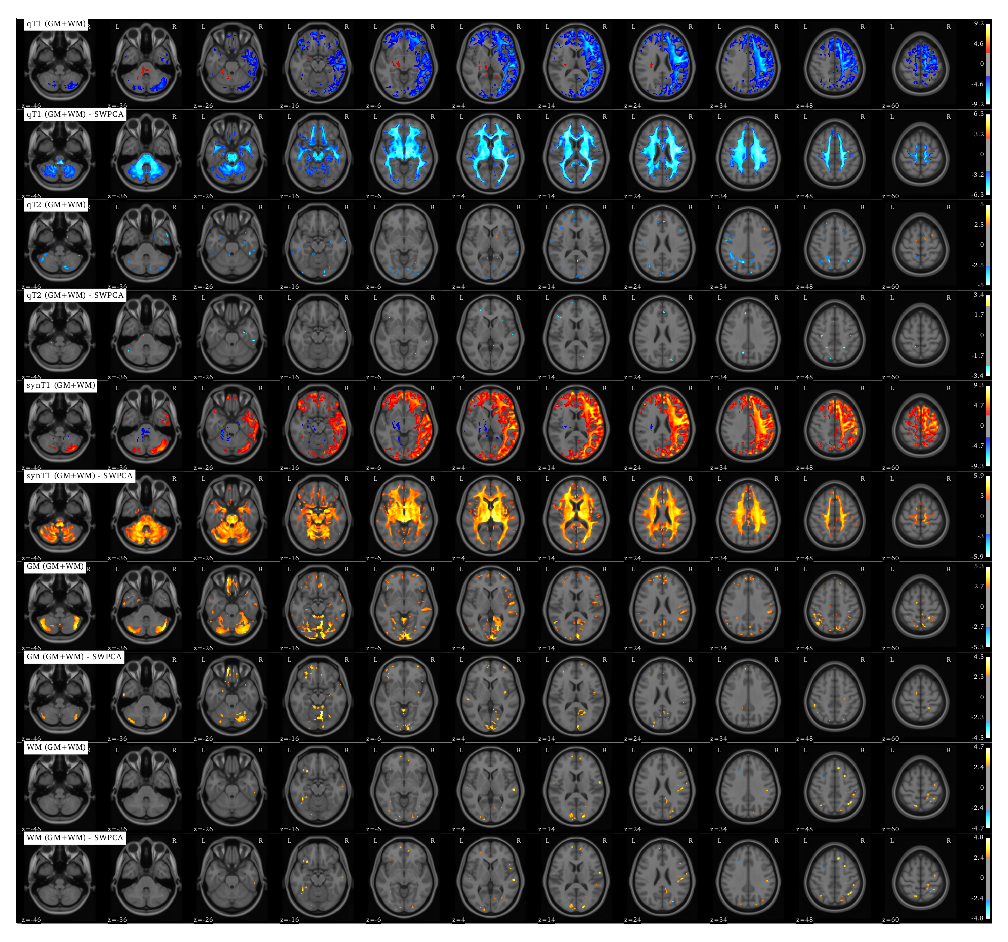
\includegraphics[width=\linewidth]{Graphics/ch7/FIGURE03}
	\caption[Brain t-map (\acs{VBM}) of significant ($p<0.01$, $|t|>2.57$) \acs{GM} and \acs{WM} between-group differences using \acs{qT1}, \acs{qT2}, \acs{synT1}, \acs{GM} and \acs{WM} modalities after applying \acs{SWPCA} to remove site effects.]{Brain t-map (\ac{VBM}) of significant ($p<0.01$, $|t|>2.57$) \ac{GM} and \ac{WM} between-group differences using \ac{qT1}, \ac{qT2}, \ac{synT1}, \ac{GM} and \ac{WM} modalities before and after applying \ac{SWPCA} to remove site effects.}
	\label{fig:swpcaFIGURE03}
\end{figure}

Performance results indicate clear advantages of using \ac{SWPCA}, in particular in the case of \ac{qT1} and \ac{synT1} which were associated with strong site-dependent variance. These results are also consistent with the reduction of significant between-group areas observed in Figure~\ref{fig:swpcaFIGURE03}.
	
The between-site differences were smaller for \ac{GM} and \ac{WM} maps, possibly due their reduced sensitivity. Since fractional occupancy values are abstract, unitless values derived from each image they are less influenced by the acquisition site effects. For \ac{qT2} maps, the site-related differences were greater for the \ac{CTL} participants than \ac{ASD} where, according to the classification accuracy, they were nearly indistinguishable. Acquisition site differences were therefore noticeably reduced in the \ac{CTL} and \all{} databases, but not in the \ac{ASD}.

\begin{bigtable}
	\begin{tabularx}{\linewidth}{ll|XX|XX|XX} 
		\multicolumn{2}{c}{} & \multicolumn{2}{c}{\spacedlowsmallcaps{\all{}}}& \multicolumn{2}{c}{\spacedlowsmallcaps{\ac{CTL}}}& \multicolumn{2}{c}{\spacedlowsmallcaps{\ac{ASD}}} \\ \cline{3-8}
		\tableheadline{Modality} & \tableheadline{Mask} & \tableheadline{no-\ac{SWPCA}} & \tableheadline{\ac{SWPCA}} & \tableheadline{no-\ac{SWPCA}} & \tableheadline{\ac{SWPCA}}& \tableheadline{no-\ac{SWPCA}} & \tableheadline{\ac{SWPCA}}\\ \toprule
		\multirow{3}{*}{\ac{qT1}} &GM+WM &		$ 0.875 \pm 0.083 $ & $ 0.530 \pm 0.130 $ & $ 0.847 \pm 0.141 $ & $ 0.543 \pm 0.115 $  &		$ 0.769 \pm 0.145 $  & $ 0.553 \pm 0.093 $ \\
		&		GM &		$ 0.849 \pm 0.085 $ & $ 0.535 \pm 0.107 $ & $ 0.835 \pm 0.154 $ & $ 0.501 \pm 0.090 $  &		$ 0.712 \pm 0.161 $  & $ 0.575 \pm 0.084 $ \\
		&		WM &		$ 0.865 \pm 0.082 $ & $ 0.447 \pm 0.071 $ & $ 0.876 \pm 0.128 $ & $ 0.441 \pm 0.058 $  &		$ 0.813 \pm 0.127 $ &  $ 0.575 \pm 0.153 $ \\
		\midrule 
		\multirow{3}{*}{\ac{qT2}} &GM+WM &		$ 0.596 \pm 0.128 $ & $ 0.503 \pm 0.093 $ & $ 0.615 \pm 0.196 $ & $ 0.454 \pm 0.075 $  &		$ 0.506 \pm 0.192 $  & $ 0.476 \pm 0.103 $ \\
		&		GM &		$ 0.596 \pm 0.126 $ & $ 0.493 \pm 0.097 $ & $ 0.549 \pm 0.187 $ & $ 0.478 \pm 0.108 $  &		$ 0.497 \pm 0.197 $  & $ 0.425 \pm 0.091 $ \\
		&		WM &		$ 0.612 \pm 0.131 $ & $ 0.560 \pm 0.128 $ & $ 0.576 \pm 0.195 $ & $ 0.550 \pm 0.146 $  &		$ 0.541 \pm 0.185 $ &  $ 0.575 \pm 0.172 $ \\
		\midrule
		\multirow{3}{*}{\ac{synT1}} & GM+WM &	$ 0.904 \pm 0.073 $ & $ 0.563 \pm 0.060 $ & $ 0.919 \pm 0.100 $ & $ 0.440 \pm 0.057 $  &		$ 0.807 \pm 0.151 $  & $ 0.631 \pm 0.098 $ \\
		&		GM &		$ 0.879 \pm 0.090 $ & $ 0.576 \pm 0.035 $ & $ 0.899 \pm 0.108 $ & $ 0.526 \pm 0.079 $  &		$ 0.800 \pm 0.145 $  & $ 0.587 \pm 0.042 $ \\
		&		WM &		$ 0.904 \pm 0.076 $ & $ 0.582 \pm 0.047 $ & $ 0.894 \pm 0.111 $ & $ 0.574 \pm 0.038 $  &	$ 0.859 \pm 0.112 $ &  $ 0.468 \pm 0.101 $ \\
		\midrule
		\multirow{2}{*}{\ac{GM}} &GM+WM &	$ 0.595 \pm 0.133 $ & $ 0.586 \pm 0.141 $ & $ 0.582 \pm 0.192 $ & $ 0.566 \pm 0.093 $  &	$ 0.481 \pm 0.169 $  & $ 0.468 \pm 0.152 $ \\
		&	GM &	$ 0.620 \pm 0.141 $ & $ 0.585 \pm 0.078 $ & $ 0.604 \pm 0.227 $ & $ 0.574 \pm 0.038 $  &	$ 0.499 \pm 0.188 $ &  $ 0.525 \pm 0.114 $ \\
		\midrule
		\multirow{2}{*}{\ac{WM}} &GM+WM &	$ 0.659 \pm 0.139 $ & $ 0.448 \pm 0.066 $ & $ 0.635 \pm 0.180 $ & $ 0.507 \pm 0.144 $  &	$ 0.522 \pm 0.206 $  & $ 0.525 \pm 0.198 $ \\
		&	WM & $ 0.639 \pm 0.124 $ & $ 0.549 \pm 0.072 $ & $ 0.578 \pm 0.194 $ & $ 0.516 \pm 0.126 $  & 	$ 0.549 \pm 0.160 $ &  $ 0.526 \pm 0.136 $ \\
		\bottomrule
	\end{tabularx}
	\caption[Between-site classification accuracy ($\pm$ standard deviation) for
	different modalities and masks without and with \acs{SWPCA} correction.]{Between-site classification accuracy ($\pm$ standard deviation) for different modalities and masks without and with \ac{SWPCA} correction.}
	\label{tab:swpcaAqSite}
\end{bigtable}

\subsection{Experiment 2: Within-site Between-Group Differences}\label{sec:swpcaE2}
In this second experiment, accuracy, sensitivity and specificity in the be\-tween-group comparison were recorded for images acquired from each site and shown at Table~\ref{tab:swpcaLONCAM}. This is an estimation of the discrimination ability of the different modalities without the influence of the site effects. For all modalities, most of the values are close to a random classifier (\~{}50\%), indicative of having either no significant differences between groups, or having spatially heterogeneous patterns of s\ac{MRI} measures across individuals where mass-univariate approaches are sub-optimal in detecting group differences. It is interesting to note that the London sample contained more between-group differences that those acquired at Cambridge. 

\begin{bigtable}
	\begin{tabularx}{\linewidth}{ll|XXX|XXX} 
		\multicolumn{2}{c}{} & \multicolumn{3}{c}{\spacedlowsmallcaps{LONDON}}& \multicolumn{3}{c}{\spacedlowsmallcaps{CAMBRIDGE}} \\ \cline{3-8}
		\tableheadline{Modality} & \tableheadline{Mask} & \tableheadline{acc.} & \tableheadline{sens.} & \tableheadline{spec.} & \tableheadline{acc.} & \tableheadline{sens.} & \tableheadline{spec.}\\ \toprule
		\multirow{3}{*}{\ac{qT1}} &GM+WM &
		$ 0.603 \pm 0.175 $ & $ 0.512 \pm 0.260 $ & $ 0.692 \pm 0.237 $ & $ 0.504 \pm 0.193 $ & $ 0.492 \pm 0.276 $ &  $ 0.515 \pm 0.307 $ \\
		&		GM &		$ 0.501 \pm 0.157 $ & $ 0.440 \pm 0.244 $ & $ 0.565 \pm 0.245 $ & $ 0.484 \pm 0.201 $ & $ 0.488 \pm 0.300 $  & $ 0.480 \pm 0.327 $ \\
		&		WM &		$ 0.505 \pm 0.174 $ & $ 0.485 \pm 0.248 $ & $ 0.526 \pm 0.242 $ & $ 0.451 \pm 0.197 $ & $ 0.465 \pm 0.297 $ &  $ 0.435 \pm 0.296 $ \\
		\midrule
		\multirow{3}{*}{\ac{qT2}} &GM+WM &
		$ 0.628 \pm 0.168 $ & $ 0.535 \pm 0.246 $ & $ 0.719 \pm 0.237 $ & $ 0.467 \pm 0.181 $ & $ 0.527 \pm 0.307 $ &  $ 0.417 \pm 0.314 $ \\
		&		GM &		$ 0.539 \pm 0.149 $ & $ 0.425 \pm 0.220 $ & $ 0.654 \pm 0.222 $ & $ 0.491 \pm 0.196 $ & $ 0.548 \pm 0.316 $  & $ 0.430 \pm 0.298 $ \\
		&		WM &		$ 0.619 \pm 0.194 $ & $ 0.585 \pm 0.262 $ & $ 0.655 \pm 0.250 $ & $ 0.472 \pm 0.195 $ & $ 0.448 \pm 0.283 $ &  $ 0.492 \pm 0.290 $ \\
		\midrule
		\multirow{3}{*}{\ac{synT1}} &GM+WM &		$ 0.665 \pm 0.158 $ & $ 0.578 \pm 0.224 $ & $ 0.755 \pm 0.238 $ & $ 0.479 \pm 0.201 $ & $ 0.478 \pm 0.318 $ &  $ 0.475 \pm 0.316 $ \\
		&		GM &		$ 0.547 \pm 0.159 $ & $ 0.475 \pm 0.237 $ & $ 0.622 \pm 0.252 $ & $ 0.514 \pm 0.218 $ & $ 0.477 \pm 0.322 $  & $ 0.555 \pm 0.342 $ \\
		&		WM &		$ 0.515 \pm 0.185 $ & $ 0.520 \pm 0.288 $ & $ 0.506 \pm 0.254 $ & $ 0.509 \pm 0.209 $ & $ 0.472 \pm 0.317 $ &  $ 0.542 \pm 0.316 $ \\
		\midrule
		\multirow{2}{*}{\ac{GM}} &GM+WM &		$ 0.513 \pm 0.171 $ & $ 0.507 \pm 0.252 $ & $ 0.518 \pm 0.245 $ & $ 0.488 \pm 0.202 $ & $ 0.445 \pm 0.318 $ &  $ 0.528 \pm 0.285 $ \\
		&		GM &		$ 0.586 \pm 0.174 $ & $ 0.610 \pm 0.247 $ & $ 0.564 \pm 0.270 $ & $ 0.521 \pm 0.187 $ & $ 0.522 \pm 0.303 $ &  $ 0.535 \pm 0.289 $ \\
		\midrule
		\multirow{2}{*}{\ac{WM}} &GM+WM &		$ 0.471 \pm 0.181 $ & $ 0.455 \pm 0.245 $ & $ 0.488 \pm 0.278 $ & $ 0.489 \pm 0.206 $ & $ 0.502 \pm 0.319 $ &  $ 0.483 \pm 0.314 $ \\
		&		WM &		$ 0.465 \pm 0.174 $ & $ 0.445 \pm 0.243 $ & $ 0.484 \pm 0.268 $ & $ 0.468 \pm 0.210 $ & $ 0.488 \pm 0.292 $ &  $ 0.448 \pm 0.305 $ \\
		\bottomrule
	\end{tabularx}
	\caption[Classification accuracy (acc), sensitivity (sens) and specificity (spec) $\pm$ standard deviation for each modality and mask using the participants acquired at the \lon{} and \cam{} sites.]{Classification accuracy (acc), sensitivity (sens) and specificity (spec) $\pm$ standard deviation for each modality and mask using the participants acquired at the \lon{} and \cam{} sites.}
	\label{tab:swpcaLONCAM}
\end{bigtable}



\subsection{Experiment 3: Effect of \acs{SWPCA} on Group Differences}\label{sec:swpcaE3}
Finally, group differences were characterised with and without applying site-effects reduction via \ac{SWPCA} to the five modalities. 

Whole-brain \ac{VBM} analysis was performed on the corrected and uncorrected maps from each modality. Figure~\ref{fig:swpcaFIGURE04} depicts the brain $t$-maps of significant ($p<0.01$, $|t|>2.57$) \ac{qT1}, \ac{qT2}, \ac{synT1}, \ac{GM} and \ac{WM} between-group differences, using \all{}, with the GM+WM mask, before and after applying \ac{SWPCA}, so that the reduction of site-related variability can be observed. Some of the highlighted areas after applying \ac{SWPCA} are inconsistent across modalities, with spurious peaks and noise, including a large area around the ventricles in the \ac{qT1} and \ac{synT1} modalities related to some abnormal participants that will be discussed later. However, there were some areas that were consistent across modalities. Significant areas found across at least 4 of the 5 modalities correspond to the \ac{AAL} \cite{Tzourio-Mazoyer2002} areas of: A) right superior frontal gyrus, Brodmann area 6 (z=60); B) the pars opercularis of the left inferior frontal gyrus, Brodmann area 44; C) the pars triangularis of the left inferior frontal gyrus, Brodmann area 45; D) the posterior part of the left middle temporal gyrus (z=24); \ac{CSF} filled spaces on the margins of the ventricles (z=-6,4,14,24); and the left crus I of cerebellar hemisphere (z=-26).

\begin{figure}
	\centering
	\includegraphics[width=\linewidth]{Graphics/ch7/FIGURE04}
	\caption[Brain t-map (\acs{VBM}) of significant ($p<0.01$, $|t|>2.57$) \acs{GM} and \acs{WM} differences in \acs{ASD} using \acs{qT1}, \acs{qT2}, \acs{synT1}, \acs{GM} and \acs{WM} maps before and after applying \acs{SWPCA} to remove site effects.]{Brain t-map (\ac{VBM}) of significant ($p<0.01$, $|t|>2.57$) \ac{GM} and \ac{WM} differences in \ac{ASD} using \ac{qT1}, \ac{qT2}, \ac{synT1}, \ac{GM} and \ac{WM} maps before and after applying \ac{SWPCA} to remove site effects.}
	\label{fig:swpcaFIGURE04}
\end{figure}

The complementary \ac{CBM} (see Section~\ref{sec:swpcaEval}) analysis was performed on the most significant components. The resulting regions, statistically thresholded with $Z>2.57$ (corresponding to $p<0.01$), were superimposed on the \ac{MNI} template, and are depicted in Figure~\ref{fig:swpcaFIGURE05}. A reduction of significant between-group areas after applying \ac{SWPCA} is evident in most modalities, but particularly noticeable in the \ac{qT1} and \ac{qT2}. In \ac{WM} no significant regions were observed, neither before nor after \ac{SWPCA}. The significant regions identified in any modality corresponded to the \ac{AAL} areas of the \ac{CSF} filled areas around the ventricles (planes z=-6, 4, 14, 24), the right middle temporal gyrus (plane z=14) and the left crus I of cerebellar hemisphere (plane z=-26). However, none of these regions were repeated over more than two of the modalities, except for the large areas around ventricles that were caused by abnormalities in three participants, which will be discussed later.

\begin{figure}
	\centering
	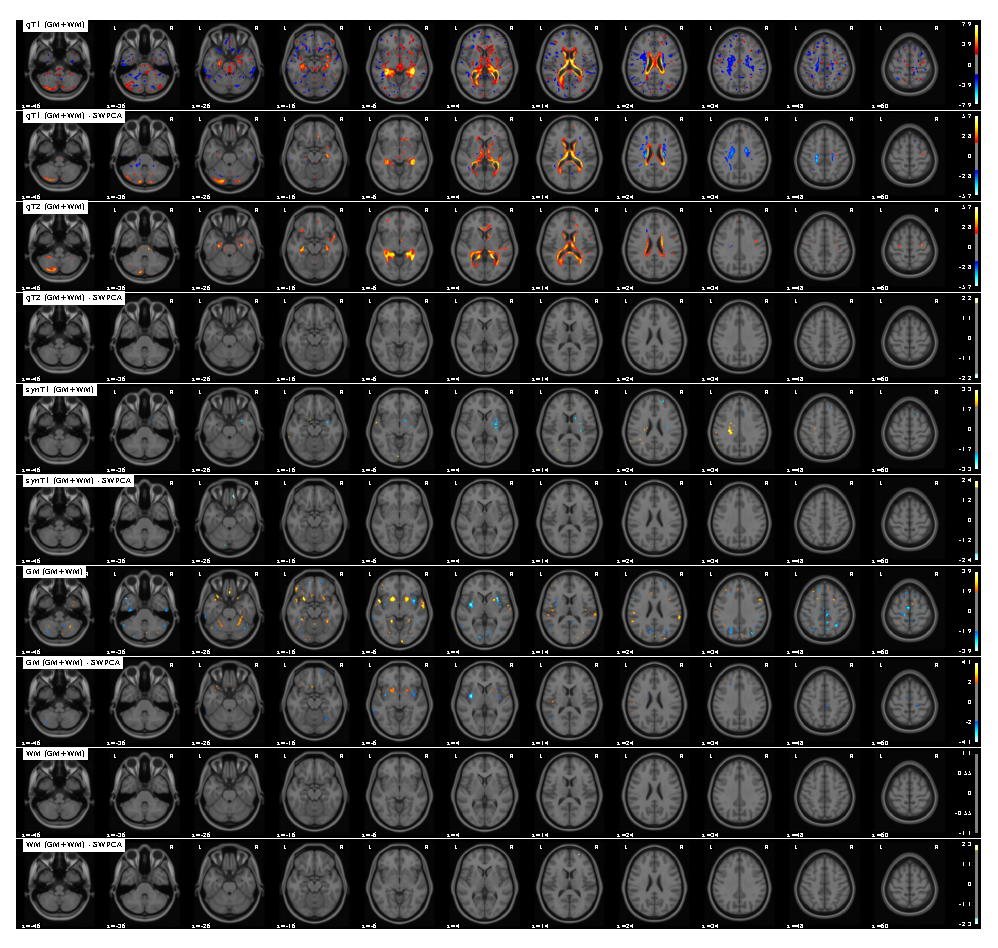
\includegraphics[width=\linewidth]{Graphics/ch7/FIGURE05}
	\caption[Brain Z-map (\acs{CBM}) of significant ($p<0.01$, $|t|>2.57$) \acs{GM} and \acs{WM} differences using \acs{qT1}, \acs{qT2}, \acs{synT1}, \acs{GM} and \acs{WM} maps before and after applying \acs{SWPCA} to remove site effects.]{Brain Z-map (\ac{CBM}) of significant ($p<0.01$, $|t|>2.57$) \acs{GM} and \acs{WM} differences using \ac{qT1}, \ac{qT2}, \ac{synT1}, \ac{GM} and \ac{WM} maps before and after applying \ac{SWPCA} to remove site effects.}
	\label{fig:swpcaFIGURE05}
\end{figure}

Performance results for the classification analysis applied to \all{} are shown in Table~\ref{tab:swpcaALL}. Between-group results were quite similar before or after applying \ac{SWPCA}, although reducing between-site variance generally reduced the performance towards a random classifier. The results in this table match the overall effects that were found in Figure~\ref{fig:swpcaFIGURE04}, where most spurious significance peaks disappeared after applying \ac{SWPCA}, but some regions were highlighted. These regions, where \ac{SWPCA} did not seem to eliminate the significant areas but enhanced them, could be responsible for the accuracy increment in the analysis of the \ac{qT2} modality, and the \ac{GM} with \ac{GM} mask.

\begin{bigtable}
	\begin{tabularx}{\linewidth}{ll|XXX|XXX} 
		\multicolumn{2}{c}{} & \multicolumn{3}{c}{\spacedlowsmallcaps{no-\ac{SWPCA}}}& \multicolumn{3}{c}{\spacedlowsmallcaps{\ac{SWPCA}}} \\ \cline{3-8}
		\tableheadline{Modality} & \tableheadline{Mask} & \tableheadline{acc.} & \tableheadline{sens.} & \tableheadline{spec.} & \tableheadline{acc.} & \tableheadline{sens.} & \tableheadline{spec.}\\ \toprule
		\multirow{2}{*}{\ac{qT1}} &GM+WM &
		$ 0.564 \pm 0.123 $ & $ 0.503 \pm 0.179 $ & $ 0.625 \pm 0.177 $ & $ 0.435 \pm 0.123 $ & $ 0.499 \pm 0.181 $ &  $ 0.371 \pm 0.178 $ \\
		&
		GM &
		$ 0.523 \pm 0.112 $ & $ 0.468 \pm 0.162 $ & $ 0.580 \pm 0.192 $ & $ 0.458 \pm 0.120 $ & $ 0.477 \pm 0.187 $ &  $ 0.441 \pm 0.210 $ \\
		&
		WM &
		$ 0.504 \pm 0.131 $ & $ 0.475 \pm 0.191 $ & $ 0.533 \pm 0.194 $ & $ 0.484 \pm 0.123 $ & $ 0.511 \pm 0.179 $ &   $ 0.456 \pm 0.194 $ \\
		\midrule
		\multirow{2}{*}{\ac{qT2}} &GM+WM &
		$ 0.578 \pm 0.115 $ & $ 0.487 \pm 0.208 $ & $ 0.669 \pm 0.178 $ & $ 0.593 \pm 0.136 $ & $ 0.546 \pm 0.206 $ &  $ 0.640 \pm 0.194 $ \\
		&
		GM &
		$ 0.554 \pm 0.135 $ & $ 0.492 \pm 0.194 $ & $ 0.614 \pm 0.181 $ & $ 0.526 \pm 0.144 $ & $ 0.512 \pm 0.209 $ &  $ 0.543 \pm 0.222 $ \\
		&
		WM &
		$ 0.516 \pm 0.138 $ & $ 0.508 \pm 0.198 $ & $ 0.522 \pm 0.216 $ & $ 0.499 \pm 0.137 $ & $ 0.477 \pm 0.209 $ &   $ 0.521 \pm 0.196 $ \\
		\midrule
		\multirow{2}{*}{\ac{synT1}} &GM+WM &
		$ 0.596 \pm 0.132 $ & $ 0.509 \pm 0.194 $ & $ 0.680 \pm 0.172 $ & $ 0.577 \pm 0.130 $ & $ 0.479 \pm 0.208 $ &  $ 0.676 \pm 0.183 $ \\
		&
		GM &
		$ 0.587 \pm 0.139 $ & $ 0.509 \pm 0.210 $ & $ 0.665 \pm 0.169 $ & $ 0.483 \pm 0.136 $ & $ 0.489 \pm 0.218 $ &  $ 0.480 \pm 0.200 $ \\
		&
		WM &
		$ 0.496 \pm 0.139 $ & $ 0.500 \pm 0.189 $ & $ 0.492 \pm 0.194 $ & $ 0.487 \pm 0.134 $ & $ 0.513 \pm 0.189 $ &   $ 0.461 \pm 0.211 $ \\
		\midrule
		\multirow{2}{*}{\ac{GM}} &GM+WM &
		$ 0.498 \pm 0.120 $ & $ 0.486 \pm 0.197 $ & $ 0.507 \pm 0.203 $ & $ 0.490 \pm 0.123 $ & $ 0.514 \pm 0.197 $ &  $ 0.465 \pm 0.182 $ \\
		&
		GM &
		$ 0.574 \pm 0.121 $ & $ 0.571 \pm 0.189 $ & $ 0.579 \pm 0.163 $ & $ 0.593 \pm 0.127 $ & $ 0.602 \pm 0.172 $ &   $ 0.587 \pm 0.190 $ \\
		\midrule
		\multirow{2}{*}{\ac{WM}} &GM+WM &
		$ 0.499 \pm 0.132 $ & $ 0.506 \pm 0.189 $ & $ 0.487 \pm 0.181 $ & $ 0.521 \pm 0.129 $ & $ 0.510 \pm 0.209 $ &  $ 0.532 \pm 0.180 $ \\
		&
		WM &
		$ 0.506 \pm 0.143 $ & $ 0.488 \pm 0.219 $ & $ 0.526 \pm 0.197 $ & $ 0.507 \pm 0.122 $ & $ 0.521 \pm 0.165 $ &   $ 0.492 \pm 0.193 $ \\
		\bottomrule
	\end{tabularx}
	\caption[Classification accuracy (acc), sensitivity (sens), and specificity (spec) $\pm$ STD for the different modalities and masks using \all{}, before and after applying \acs{SWPCA}.]{Classification accuracy (acc), sensitivity (sens), and specificity (spec) $\pm$ STD for the different modalities and masks using \all{}, before and after applying \ac{SWPCA}.}
	\label{tab:swpcaALL}
\end{bigtable}

\section{Discussion}
Brain anatomical and functional differences between \ac{ASD} participants and controls have been explored by a number of previous studies \cite{DiMartino2014,Ecker2015,Hernandez2015,Lenroot2013,Zuercher2015}. Many affected structures have been proposed in each of these studies, however as a recent large-scale study points out \cite{haar2014anatomical}, these are frequently inconsistent throughout the literature. Researchers argue that most of these structures are database-dependent, and since many studies use multi-site acquisition procedures, the variance introduced by each acquisition site is a probable source of Type I errors. 

The technical and logistical drawbacks of multicentre studies are widely documented, including participant recruitment procedures \cite{Pearlson2009} and technical effects that range from the usage of different equipment or acquisition parameters \cite{VanHorn2009} to physical changes that affect the performance of \ac{MRI} scanners across time \cite{Pearlson2009}. There is general recognition that standardization is needed to ensure the uniformity of the acquired maps. Different approaches have been used in large-scale studies, such as \ac{ADNI} where human ``phantoms'' were used to perform a preparatory optimisation of \ac{MRI} scanning platforms \cite{friedman2006report}. 

There are two major types of site effects, regardless of their source: geometric distortions and intensity inhomogeneities. In this work, we focused on the latter, since much of the geometric distortion has been eliminated during acquisition (see Section~\ref{sec:aims-mri}), and the DARTEL normalization and registration acts as a homogenizing step, reducing both between-site and between-subject geometric differences, substantially reducing their impact.

Regarding intensity correction, in the \ac{MRC-AIMS} database used in this study \cite{Ecker2012,Ecker2013}, a standardization procedure based on quantitative imaging \cite{deoni2008standardized} was used to minimize inter-site variance and improve the signal-to-noise contrast. However, as the between-site analysis in Section~\ref{sec:swpcaE1} suggests, this strategy still results in variance that makes it easier to distinguish scanning sites than diagnostic groups. For example, when using \ac{qT1} the accuracy for \lon{} vs. \cam{} classification was {\textgreater}80\%, whilst when classifying \ac{ASD} vs. \ac{CTL} it was 52\%. This marks the substantial effect of site variance on the maps' intensity distribution, even when the multi-site study employs quantitative imaging protocol on the same model of scanner platform across sites. However, with the inclusion of \ac{GM} and \ac{WM} maps, we can observe that the inhomogeneities found on \ac{qT1} or \ac{synT1} barely affected the segmentation procedure. 

In this work, the approach we have taken is to perform a multivariate decomposition of each dataset into a number of components that explain different portions of variance. The following step was to identify the components of variance that are due to multi-site acquisition and reduce them. Decomposition was completed using \ac{PCA} and then, to identify which of the components were linked to acquisition site, we performed an \ac{ANOVA} on the component scores. Finally, using the weighting function defined in Sec.~\ref{sec:swpcaE3}, we reconstructed the original signal reducing the undesired variance, in what we called \ac{SWPCA}. The method has proven its ability in reducing undesired variance, quantifiable by means of the accuracy obtained in a site vs. site classification. In this case, \ac{SWPCA} reduced the accuracy from {\textgreater}0.8 to approximately $\approx0.5$, a random classifier, suggesting that most site-related variance was eliminated. 

A simpler approach such as applying a voxel-by-voxel \ac{ANOVA} would also be useful to reduce the acquisition site effects \cite{Suckling2012}. However, \ac{SWPCA} is a multivariate approach that still offers major advantages over this voxel-wise algorithm, and similar algorithms have found utility in text document searches \cite{Kriegel2008,tavoli2013}. First, \ac{PCA} models the different sources of variance of the dataset, whereas a simple voxel-wise \ac{ANOVA} only removes mean site differences, which might result in less statistical power. Secondly, \ac{SWPCA} is multivariate in nature, where each component contains information that potentially affects all voxels. Together, these two features allow \ac{SWPCA} to identify the components linked to the undesired effects, and reduce their impact with a weighted reconstruction approach, reducing the general variance related to the acquisition site. However, this increased power reveals a major drawback: \ac{SWPCA} needs at least a moderate number of participants to work properly. That is the reason why we cannot apply \ac{SWPCA} to databases such as \ac{ADNI} \cite{friedman2006report} or ABIDE \cite{DiMartino2014}, where the number of participants acquired at each site is small, or to the six travelling phantoms used in the calibration of the \ac{MRC-AIMS} study. 

There exist a number of similar multivariate methods that model the influence of categorical variables, such as the well-known \ac{PLS} algorithm \cite{vinzi2010} or \acf{SVA} \cite{Leek2007}. In the first case, both \ac{PLS} and \ac{SWPCA} take categorical variables $\mathbf{Y}$ along with the data $\mathbf{X}$ as inputs to partition the influence of these into components. However, the most significant difference is the underlying model. Whilst \ac{SWPCA} estimates the principal components blindly using their variance, which is what we aim to reduce, and performs an \ac{ANOVA} afterwards, \ac{PLS} uses the categorical variable in the computation of the covariance matrix and then estimates the components. 


On the other hand, \ac{SVA}, used for gene expression studies \cite{Leek2007}, is more comparable to \ac{SWPCA}. The \ac{SVA} algorithm uses a number of decomposition and significance estimation steps to construct a set of surrogate variables; that is, variables that account for the unmodeled variance and expression heterogeneity. While similar to \ac{SWPCA} in the steps used (i.e. \ac{SVD} decomposition and significance estimation), their approaches are fundamentally different. \ac{SVA} constructs a higher complexity model that starts by eliminating the contribution of primary variables to produce a number of unknown hidden (surrogate) variables, whereas \ac{SWPCA} is intended to reduce complexity by producing variance-reduced maps to reduce the influence of previously known, but unconsidered, variables and facilitate a subsequent analysis focused only on the relevant variables.

\begin{figure}
\centering
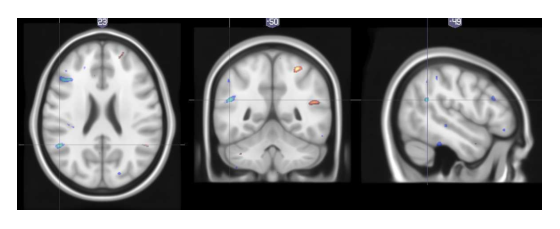
\includegraphics[width=0.7\linewidth]{Graphics/ch7/FIGURE06}
\caption[Location of hte singifcant region labelled D (posterior part of the superior temporal gyrus) within the \acs{MNI} template.]{Location of hte singifcant region labelled D (posterior part of the superior temporal gyrus) within the \acs{MNI} template.}
\label{fig:figure06}
\end{figure}

Focusing on the \ac{VBM} results, after performing the site-effects removal by \ac{SWPCA} significant between-group differences were noted in five areas: A) the right superior frontal gyrus; B) the pars opercularis of the left inferior frontal gyrus; C) the pars triangularis of the left inferior frontal gyrus; D) the posterior part of the left middle temporal gyrus; and E) the left crus I of cerebellar hemisphere. The first three regions are within Brodmann areas 6, 44 and 45. However, when examining the projection of the region D onto the \ac{MNI} template (see Figure~\ref{fig:figure06}), it is also located in the posterior part of the left superior temporal gyrus. Therefore, D corresponds closely with the region between Brodmann areas 22 and 39, the Temporo-Parietal Junction (TPJ), with negative t-value at the left side (containing Wernicke's area) and positive t-value at the right side. 

The role of these regions in autism has received much attention. Brodmann areas 44 and 45, that together make the Broca's Area (of importance in speech production and a proposed part of the human mirror neuron system \cite{Nishitani2005}), is a region where mirror neuron dysfunction has been consistently reported in \ac{ASD}-affected children \cite{Dapretto2006} and adults \cite{Hadjikhani2006,Lopez-Hurtado2008,Verly2014}. Wernicke's area, contained in the left TPJ, is also linked to language, and has been associated with \ac{ASD} in several works \cite{Hadjikhani2006,Verly2014}. Additionally, the right TPJ has been proposed as related to mentalizing and has been repeatedly implicated in autism \cite{Barnea-Goraly2004}, including a f\ac{MRI} study of a subsample of this same AIMS dataset \cite{Lombardo2011}. The right superior frontal gyrus (region A) is more equivocal, with some studies \cite{Ecker2010,Ecker2012} reporting abnormalities in this area, while others \cite{Hadjikhani2006,Segovia2014} report no significant differences. Our analyses reveal no differences in the insula and amygdala, brain structures frequently linked to autism. 

\begin{figure}
	\centering
	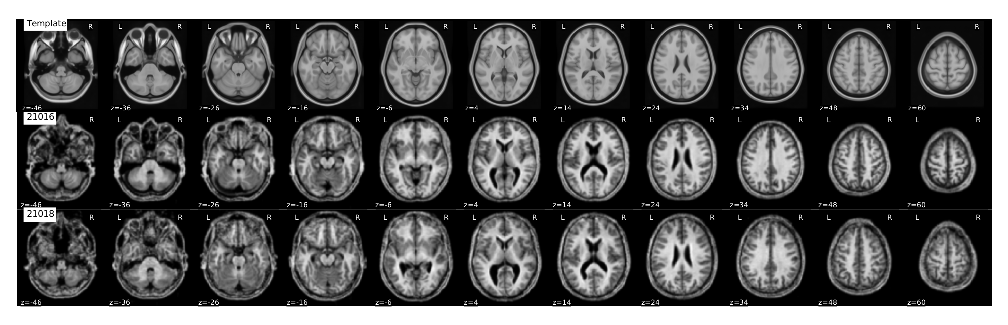
\includegraphics[width=\linewidth]{Graphics/ch7/FIGURE07}
	\caption[The template used in this work compared to two of the participants with abnormal ventricle size (21016 and 21018).]{The template used in this work compared to two of the participants with abnormal ventricle size (21016 and 21018). Atrophy of the cerebellum in participant 21016 can also be appreciated, responsible for some of the `highlighted' areas in \acs{qT1}, \acs{qT2} and \ac{synT1} $t$-maps (see Fig.~\ref{fig:swpcaFIGURE04}).}
	\label{fig:swpcaFIGURE07}
\end{figure}

Some regions, particularly in \ac{qT2}, \ac{synT1} and segmented \ac{GM} maps show potentially spurious significance peaks around the ventricles and especially in the left crus I of cerebellar hemisphere (region E). After examining the database, two individuals had appreciable structural abnormalities in the form of abnormal ventricle size and cerebellar atrophy, as can be seen in Figure~\ref{fig:swpcaFIGURE07}. It is possible that these participants influenced the computation of the $t$-maps, and therefore are responsible for the significance in region E and areas surrounding the ventricles and, since they are part of the \lon{} subdataset, could also be responsible for the increased classification accuracy of the quantitative T1 and T2, and the synthetic T1 maps in this sub-dataset.

After observing the influence of these participants on the computation of the $t$-maps, we can assume that most of the structural differences in \ac{ASD} are so subtle that the influence of just one or two images can impact on the final results. This, along with the poor performance of the classification pipeline presented in Section~\ref{sec:swpcaEval}, dramatically reduces the significance of the aforementioned $t$-maps. Therefore, the existing evidence leads to the conclusion that \ac{ASD} presents as either undetectable structural differences or, more likely, with such heterogeneous differences that are difficult to establish a common pattern even after reducing the variance introduced by acquisition site. 

It may be the case that cohorts of individuals examined at different sites are somehow systematically biased towards a specific type of patient (in ways that we cannot see simply based on phenotypic information), then site-related intensity variability is also enriched with important variability about nested autism subgroups. So with any technique trying to remove the site-related inhomogeneity, the subgroup information could also be removed. Together, the evidence supports the claim that defining meaningful subgroups based on different measures, such as genetic profiling, clinical co-morbidities or sensory sensitivities, is the most urgent next step for \ac{ASD} research \cite{haar2014anatomical}. 
	